\documentclass[Report.tex]{subfiles}
\externaldocument[I-]{chapter_1_introduction}
\externaldocument[M-]{chapter_2_method}
\externaldocument[R-]{chapter_4_result}
\externaldocument[C-]{chapter_5_conclusion}
\externaldocument[RE-]{chapter_6_recognition}

\begin{document}
\chapter{Discarded Method}
\label{chap:Discarded Method}
\section{Description}
This chapter covers the methods tried but not included in the end result, because they showed dissatisfactory results. This chapter is also organized like Chapter~\ref{chap:Method}, but for component description please refer to the previous chapter.

\section{Text Segmentation}
We tried to expand the original approach to be able to detect text with noise, natural images. We tried Stroke Width Transform first, then OpenCv scene text detection. We abandon both approach because of time constrain and difficulties of implementation. We decided therefore to focus on other part of the project first.

\begin{flushleft}
  \subsubsection{Other Method 1: Stroke Width Transform}
  We tried Stroke Width Transform to do Text Segmentation when original approach gave a decent result. It was original propose by Epstein et al 2010 \cite{epshtein_stroke_2010}. Since OpenCv do not have this implemented we tried to implement it ourself. Additional sources was used in our attempt to implement it\cite{werner_text_????, _c++_????, bunn_strokewidthtransform:_2018}. We was not able to finish this, but think we should mention it since we spend some time on it. The steps of Stroke Width Transform is as followed:
  \begin{enumerate}
    \item \textbf{Edge Detection and edge orientation(Done)}
    We need to have Edge image and orientation of the gradient image.
    Canny and Sobel was used in the original paper and other sources. This is simple since OpenCv have both Canny and Sobel implemented.
    \item \textbf{Stroke Width Transform(Done)}
    Here we had to do more. We have to find a line from a starting point and the angle. We was able to implement this part, but was some uncertainties. It only work on black text with white background. That is because the orientation(Sobel filtering) are dependent on it. The paper talk about doing a second pass with inverse image, but we decided to ignore it, in order to come farther in the algorithm.
    \item \textbf{Find Connected Component(Done)}
    In this point we are find connect component. The caveat here is the components need to be connected with regards to the Stride Length. We used 'One Component At A Time' algorithm to find all the different components. This part we was able to finish.
    \item \textbf{Exclude noise and find letters(not Done)}
    Since Stroke Width Transform tend to make a lot of noise. The obvious one is making single lines. This part are suppose to exclude this noise and at the same time exclude anything that is not a letter.The theory is, since letter and text all usually have the same stroke width, we can use this information do estimate what is letter and what is not. We was not able to finish this part.
    \item \textbf{Find lines/words(not Done)}
    Was not able to get to this part, but ideal it will combine letters to a single line or words.
  \end{enumerate}
  In cases where the image have a lot of non text object, it will work fine with it. We ended up discarding this approach since it was to time consuming and decided on working on simple approach first.
\end{flushleft}

\begin{flushleft}
  \subsubsection{Other Method 2: OpenCv Scene Text Detection}
  OpenCV have it own Text Scene Detection. The approach of this algorithm is to detect text in scene using Classifier and Components Tree, propose by Lukás Neumann \& Jiri Matas \cite{neumann_real-time_2012}. Since we already discarded Stroke Width Transform to focus on simple approach, we decided not use it. We had some problem to get propel result as well.
\end{flushleft}

\begin{figure}[ht]
  \centering
  \begin{subfigure}[t]{4cm}
    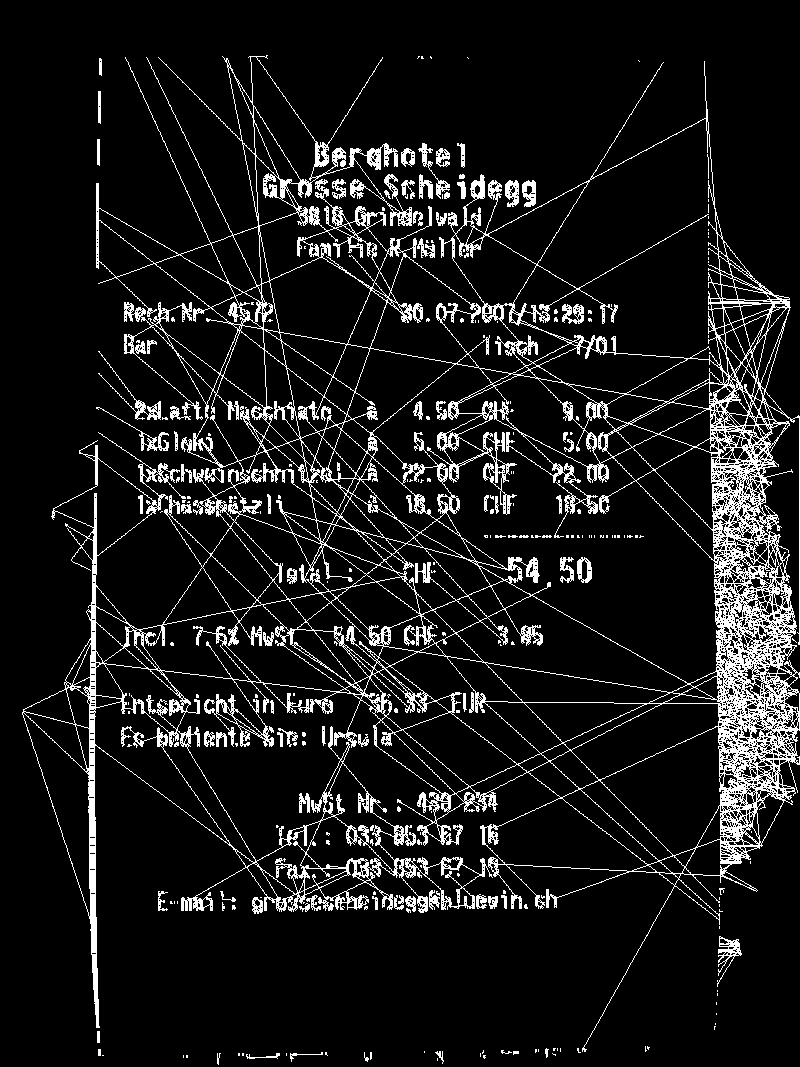
\includegraphics[width=3cm]{res/swt.png}
    \caption{Unfinished SWT}
  \end{subfigure}
  \hspace{5mm}%
  \begin{subfigure}[t]{4cm}
    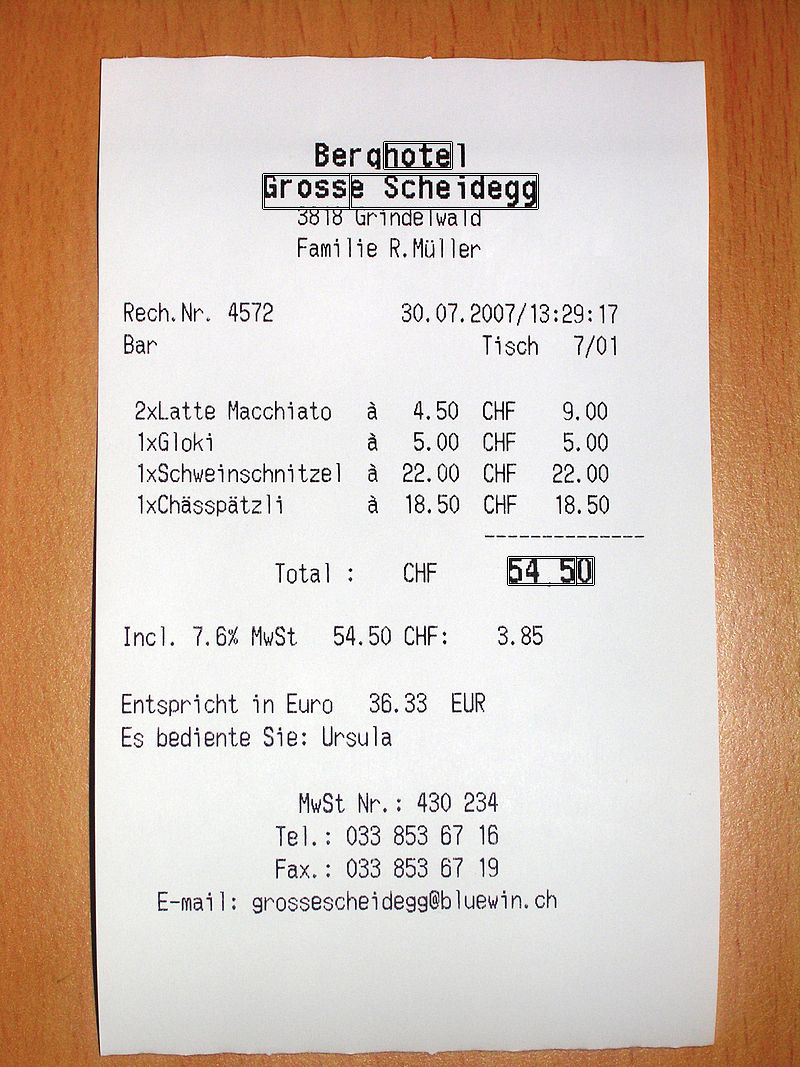
\includegraphics[width=3cm]{res/OpenCV_Std.png}
    \caption{OpenCv Scene text detection}
  \end{subfigure}
  \hspace{5mm}%
  \caption{Result of Discarded Segment Text Method}
  \label{fig:Text_detection_result}
\end{figure}

\section{Preprocessing}
\subsection{Find rotation}
\label{Discard:rotation}
\begin{flushleft}
  \textbf{Approach: OpenCV minAreaRect() + CNN solution} \\
  This approach is the same as final approach, only we added a additional step with CNN to classify wrong angle rotation. Our method returns text rotated in one of following angles [0\textdegree, 90\textdegree, 180\textdegree, 270\textdegree], see Figure~\ref{fig:4angle_rot}for illustration. We will use a CNN to determine which of the angles is correct and then rotate it accordingly.
  To train the network we needed a dataset with the corresponding angles as labels, as we could not find one, we decided to create it ourself. We discarded it because it gave only a 60\% accuracy of the right angle, and we are only working on simple text images with little skew. The approach is described below: 
  \begin{enumerate}
    \item \textbf{OpenCV minAreaRect()}
    The same approach mention in section \ref{Method:Preprocessing} find rotation
    \item \textbf{CNN solution - find correct rotation}
    Now that we have text rotated in one of [0\textdegree, 90\textdegree, 180\textdegree, 270\textdegree], we have several options finding the correct angle of the text segment.
    \begin{enumerate}
      \item{The most straightforward approach would be to find the rotation of first character and rotate the whole segment accordingly (fast and naive)}
      \item{Pick N characters and find their rotation, angle with most matches will be our final angle of rotation. This is somewhat slower (depends on N) but gives us bit more confidence than (a)}
      \item{Finally we can classify the angle of each individual character before we try to determine the correct angle based on the results. This gives us the highest accuracy but on the cost of time/computation power. This is the only approach able to successfully recognize this type of text: (find better example)\LaTeX}
      \end{enumerate}
    \end{enumerate}

    \begin{figure}[H]
      \centering
      
\includegraphics[height=4cm]{res/4angle_rot.png}
      \caption{cv.minAreaRect cannot differentiate between 0\textdegree and 180\textdegree, and 90\textdegree and 270\textdegree}
      \label{fig:4angle_rot}
    \end{figure}

\end{flushleft}


\begin{flushleft}
  \textbf{Approach: Hough Transform} \\
  \href{https://en.wikipedia.org/wiki/Hough_transform}{Hough transform} is a well known algorithm to find lines, its approach is to see if it can align some threshold of pixels on one straight line. To help with this process we will do a simple edge detection algorithm on the image before running it through the Hough Transform. \par Bellow, the steps needed to perform this approach are mentioned.

  \begin{enumerate}
    \item \textbf{Edge detection}
    Too make the Hough transform perform better we want to remove unnecessary noise. Canny edge detection algorithm is a robust and fast solution for this.
    \item \textbf{Line detection}
    Now perform the actually Hough Transform.
    \item \textbf{Rotate image}
    Lastly we need to rotate the image according to the lines from the Hough Transform.
  \end{enumerate}
\end{flushleft}

\subsection{Character Segmentation}
Since we used Projection Histogram to fine line, we can use it to fine character segment as well. We started initially to do that, but later switch to the new approach. The approach is similar to Line detection in section \ref{subsec:Find_line}. It weakness is that we may not get the right height of each character, meaning we get more background. See figure \ref{fig:Project_histogram}


\section{Classification}
\label{sec:Discarded Method:Classification}

\begin{flushleft}
  As mention in \ref{Method:Classification}, we also tried to use MLP to do classification of letter. We gave a bigger overview of the different Hyper-parameters, strength and weakness of MLP in section \ref{Recognition:subsec:MLP}. 
  We decided to avoid using MLP in our project as it required lots of training data, is not able to detect spacial or minor rotation changes, e.g. a network trained with MNIST with accuracy over 95\% was doing poorly in recognizing machine-printed characters, even though they were etalon of a perfect input.

\end{flushleft}

\section{Datasets}
\begin{flushleft}

\textbf{MNIST} was discarded as were decided to stick with machine printed digits and letters, none of which were included in MNIST. It was a good starting point to test our networks (both MLP and CNN) but it was time to move on.

\par
\textbf{ROT*} - dataset containing rotated examples of another set (*) but labels corespont to angle of rotation. In our case we only had 4 classes [0-3], one for each angle in [0, 90, 180, 270].
This set was discarded as out network showed very little learning progress as the accuracy of predictions was constantly around 65\%. Now that is not datasets fault, most likely it was due to bad network topology or poor choice of hyper parameters but we didn't had enough time to debug this part of project and decided to stick to OpenCV's minAreaRect() results.


\end{flushleft}

\end{document}
